\subsection{Experimental Settings}
\begin{itemize}
    \item CPU\::
    \item RAM\::
    \item RocksDB version\::
\end{itemize}

\subsection{Experimental Results}
Experiement results for workload
\begin{itemize}
    \item \# of Inserts \-- 500000
    \item \# of Updates \-- 250000, 500000, 750000
    \item \# of Range Queries \-- 100 
    \item Selectivity for Range Queries \-- 0.2, 0.4, 0.8
\end{itemize}

\begin{figure}
    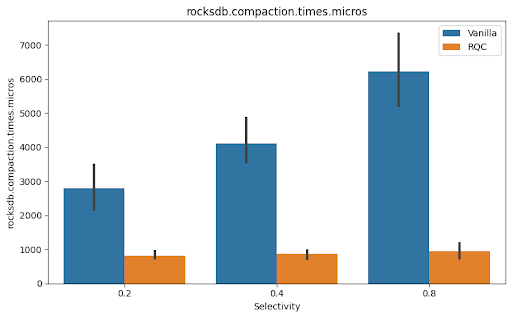
\includegraphics[scale=0.45]{Figures/Compaction Times.png}
    \caption{Number of compactions triggered during the workload execution}\label{fig:compaction_times}
\end{figure}

Figure-\ref{fig:compaction_times} shows the comparison between the number of times compaction is triggered for vanilla 
vs query-driven approach for the given workload. It appears that for different updates with different selectivity, the 
vanilla approach triggered more compactions as compared to the query-driven approach.

\begin{figure}
    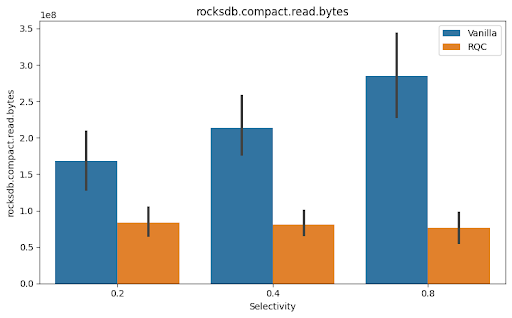
\includegraphics[scale=0.45]{Figures/Compaction Read Bytes.png}
    \caption{Number of bytes read during compactions}\label{fig:compaction_read_bytes}
\end{figure}

\begin{figure}
    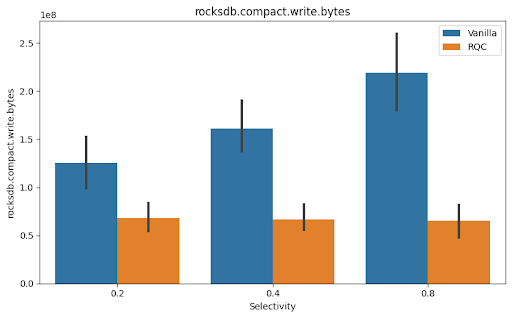
\includegraphics[scale=0.45]{Figures/Compaction Write Bytes.png}
    \caption{Number of bytes written during compactions}\label{fig:compaction_write_bytes}
\end{figure}

Figure-\ref{fig:compaction_read_bytes} \& Figure-\ref{fig:compaction_write_bytes} shows the comparison between read and 
writes bytes during the compactions that were triggered in vanilla and query-driven comapactions. We can see that the 
bytes that were read and written during the vanilla are much higher than the newer approach

\begin{figure}
    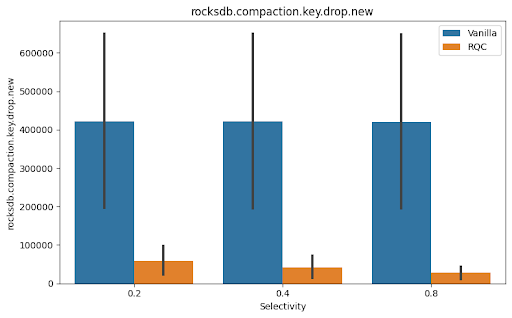
\includegraphics[scale=0.45]{Figures/Keys Drop In Compactions.png}
    \caption{Number of keys dropped during compactions}\label{fig:keys_drop_in_compactions}
\end{figure}

Figure-\ref{fig:keys_drop_in_compactions} shows the number of keys that were dropped or re-written with newer values 
while compaction.

\begin{figure}
    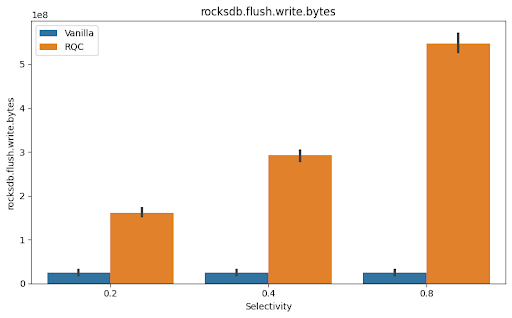
\includegraphics[scale=0.45]{Figures/Range Query Flush Write Bytes.png}
    \caption{Number of bytes written during range query and buffer flush at 
    level-0}\label{fig:range_query_flush_write_bytes}
\end{figure}

Figure-\ref{fig:range_query_flush_write_bytes} show that query-driven compaction writes more bytes while flushing
partial files and in-range files during range queries. This factor can be tuned by computing the overlapping entries in 
the lower levels while performing the range query. If the lower levels have less number of entries that overlap with the 
higher level then we can perform the vanilla fashion range query but if the overlap is much larger then we can go for 
query-driven compaction.